\section{Hearing system}
The hearing system referee to the path way of the sound wave to the nerve cell on the basilar membrane, where only the natural hearing ways is of interesting in this project. The natural hearing ways is the \gls{ac} and \gls{bc} sound way, where the airborne wave is stimulating the cochlea by moving the tympanic membrane, where the boneborne wave is stimulating the cochlea by vibration in the skull. The pathway from the tympanic membrane to the basilar membrane in the cochlea is well known and well understood, where the \gls{bc} is not completely understod \citep{stenfelt_2005} The following section will give an introduction to both the \gls{ac} and \gls{bc} hearing.


\section{Air conduction of sound}
The natural way to stimulate the nerve cell in the basilar membrane is the \gls{ac} with airborne sound. The path way from airborne wave outside the ear to the cochlea can be divided intro three path. The first path the sound wave is travelling through is the outer ear, which consist of the pinna and the ear canal. The second pathway is the middle ear where the Tympanic membrane is the membrane which convert airborne wave to mechanical movement. The middle ear consist of three auditory bone and the Eustachian tube. One bone is connected to the Tympanic membrane and one bone is connected to the oval and the last bone connect those bone together. The third pathway is the inner ear where the oval window is a membrane that convert mechanical borne wave intro liquid borne wave \citep{ho_2017}. The inner ear consist of the cochlea and the vestibular system, where the vestibular is a system for balance and do not have any hearing influence. For the hearing only the cochlea is of interest in the inner ear. The following \autoref{fig:hearing_system} shows the full hearing system.


 \begin{figure}[H]
	\centering
		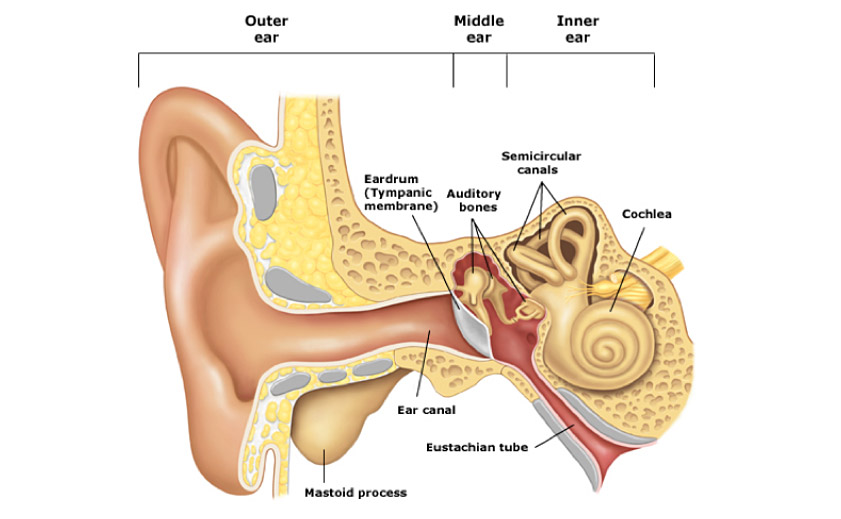
\includegraphics[width=1\textwidth]{anatomy-of-ear.jpg}
		\caption{The figure shows the outer ear, the middle ear and the inner ear.}
		\label{fig:hearing_system}
\end{figure}

\subsection{Functions for ear parts}
The pinna of the outer ear is shaped differently for every person and is very important for localisation of sound event. The shape of the pinna makes amplification, peaks and dips in the sound wave and including the ear canal the changing of the sound in the outer ear is called the \gls{hrtf}. Since the pinna is different for every person, every person have there own \gls{hrtf} and the brain have learned from birth the exact \gls{hrtf}. By changing the \gls{hrtf} on a person, the brain will be confused, but with time the brain can learn a new \gls{hrtf} if necessary. After the sound waves have entered the outer ear and changed by the pinna and the ear canal the tympanic membrane, also called the eardrum, is moving accordingly to the air pressure variation in the ear canal and transmitted to the middle ear.  

The middle ear consist of the three auditory bones, the hammer (malleus), the anvil (incus) and the stirrup (stapes), where the sound wave is travelling mechanically. The bone act as a impedance adaptation from air to liquid and have an amplification of approximation 20 times. The Eustachian tube function is to equalise the air pressure on both side on the eardrum. A build up pressure in the middle ear will affect the hearing negatively. The bone Mallus is attached to the oval window where stapes is attached to the tympanic membrane.

Vibration of the oval window cause wave travelling in the cochlea fluids, those fluid borne wave makes the basilar membrane to vibrate because pressure difference between the cochlear perilymphatic \citep{ho_2017}. The vibration of the basilar membrane gets the inner hair cell to move and generate electric response signal that is transmitted through the auditory nerve to the brain.



\section{bone conduction of sound}

For bone conduction there are reported five path way for sound vibration. First the sound can be transmitted via external auditory canal sound radiation. Secondly the inertia of the ossicular chain. Third the inertia of the cochlear fluid. Forth the compression of cochlear walls. The last transmission path is the pressure transmission from the cerebrospinal fluid (Bone conduction hearing in congenital aural atresia, https://link.springer.com/article/10.1007/s00405-015-3727-1) When using bone conduction on the skull, the fluid might also be one of the path way, and can not be let out. 
%https://www.sciencedirect.com/science/article/pii/S0003682X16304297#b0105

 \begin{figure}[H]
	\centering
		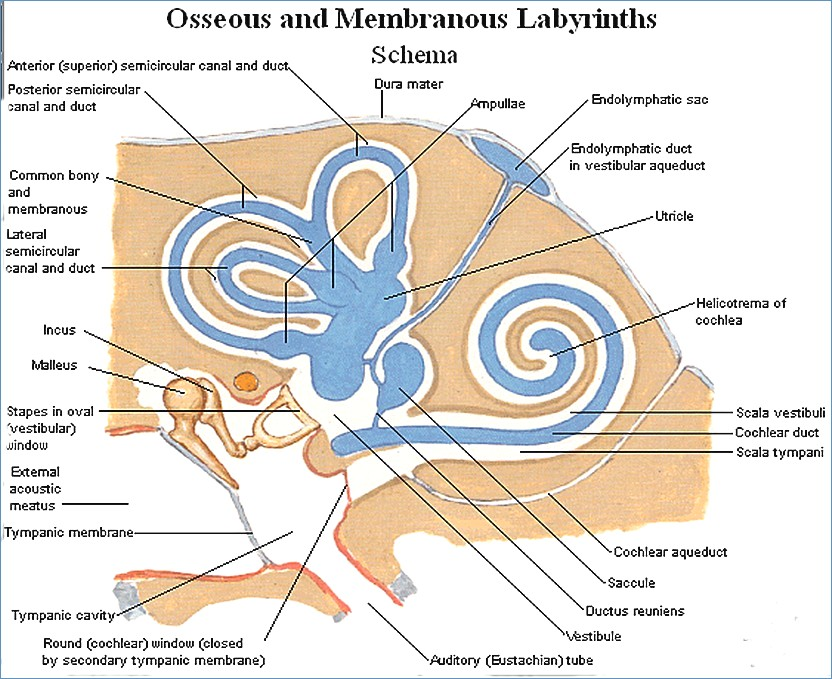
\includegraphics[width=1\textwidth]{more-on-the-vestibular-system-of-anatomy-of-cochlear-aqueduct.jpg}
		\caption{The figure shows the outer ear, the middle ear and the inner ear in detail}
		\label{fig:hearing_system_detail}
\end{figure}

 \begin{figure}[H]
	\centering
		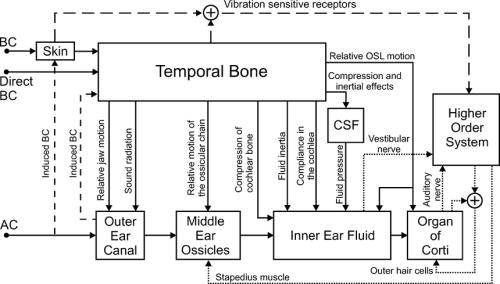
\includegraphics[width=1\textwidth]{ovidweb}
		\caption{The figure shows the transmission path for \gls{bc} \citep{stenfelt_2005}}
		\label{fig:hearing_system_pathway}
\end{figure}

